%%%%%%%%%%%%%%%%%%%%%%%%%%%%%%%%%%%%%%%%%%%%%%%%%
%
%     Chapter 5
%
%%%%%%%%%%%%%%%%%%%%%%%%%%%%%%%%%%%%%%%%%%%%%%%%

\chapter{Implementation}
\label{five}

In this Chapter, we will describe our realization of Parabix technology inside LLVM facility. LLVM is a well-structured open source compiler tool chain which is under rapid development. So during our implementation, we tried our best to follow its design principle while keeping our code modularized and isolated to be able to easily integrate with new versions of LLVM, which is evolving quickly.  Our goal of code design is to:
\begin{enumerate}
  \item Share general strategies between different targets.
  \item Utilize target-dependent operations to optimize performance.
  \item Put our code in auto-generated, thorough test.
\end{enumerate}

Most of our code sits in LLVM Target-Independent Code Generator\cite{llvm_code_gen}. From Chapter~\ref{four}, we know that current type legalization process of LLVM have big performance penalty for small element vectors, so our approach would mark $i1$, $i2$ and $i4$ vector legal type first, and then handle them in Legalize Operation Phase. For convenience, we name this set of vector types \textit{Parabix Vector}.

We walk through the following steps to mark a type legal on a certain target:
\begin{itemize}
  \item \textbf{Add new register class in target description file.} LLVM uses TableGen (.td files) to describe target information, which allows the use of domain-specific abstractions to reduce repetition \cite{llvm_code_gen}. Registers are grouped into register classes which would further tie to a set of types. We introduced GR32X for 32-bit general register like EAX, EBX for $v32i1$, GR64X for 64-bit general register like RAX, RBX for $v64i1$, VR128PX for 128-bit vector register like XMM0 to XMM15 for $v64i2$, $v32i4$, \ldots Types within the same register class can be bitcasted from one to the other, since they can actually reside in the same register.

  \item \textbf{Set calling convention.} They are two kinds of calling convention to set: return value and argument calling convention. For example, we instruct LLVM to assign $v64i2$ type return value to XMM0 to XMM3 registers, assign $v64i2$ argument type to XMM0 to XMM7 registers if we have SSE2 or to 16-byte stack slots otherwise.
\end{itemize}

Now Legalize Type Phase would recognize our $i1$, $i2$, $i4$ vectors as legal and pass them onto Legalize Operation Phase. We have two major methods to handle $i2^k$ vectors here: \textit{Custom Lowering} and \textit{DAG Combining}.

\begin{figure}[ht!]
\centering
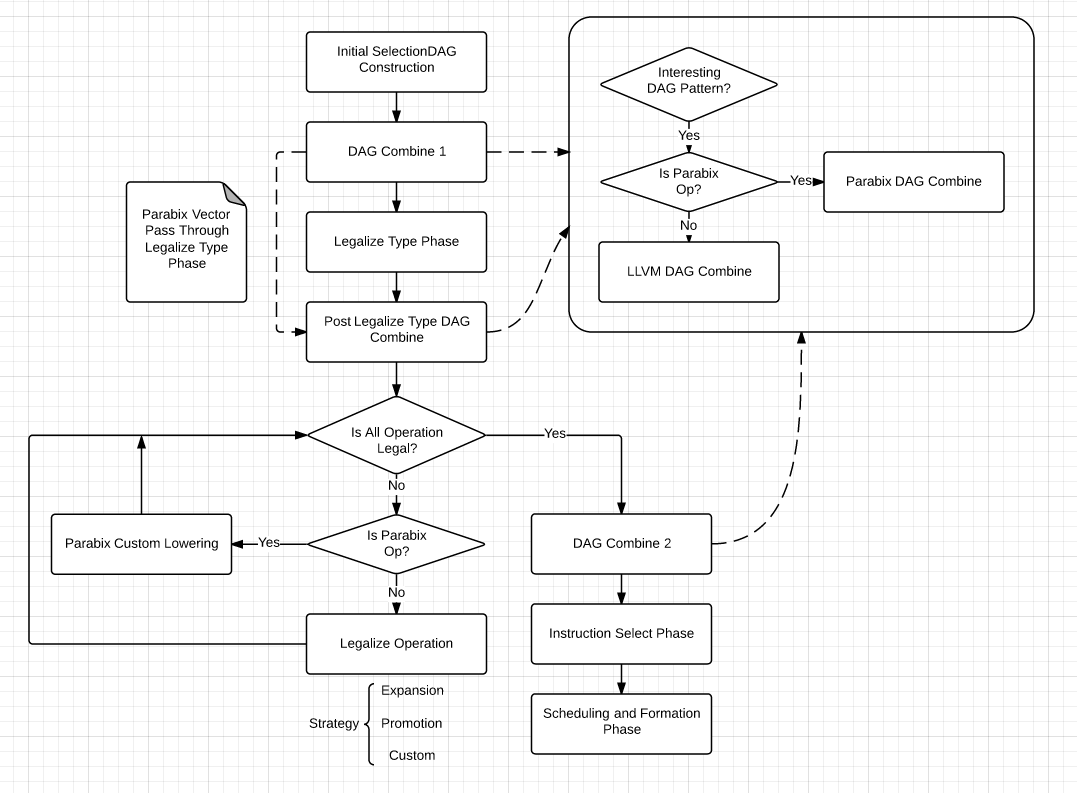
\includegraphics[width=140mm]{draw/system.png}
\caption[System overview: modified instruction selection process]{Overview of the modified instruction selection process. Logic for Parabix vectors are hooked into two places: Legalize Operation Phase and DAG Combiner. Parabix Custom Lowering and Parabix DAG Combine are modularized and separated from target-specific lowering logic.}
\label{figure:system}
\end{figure}

Figure~\ref{figure:system} gives an overview of our implementation. LLVM does operation legalization by iteration, which allows to introduce new illegal operations. Our code put hooks in target-specific lowering logic that every time it sees an illegal operation, it will check if it is parabix operation and redirects to Parabix Custom Lowering module. This module can be shared with different targets to allow general strategies. The same is true for Parabix DAG Combine. We can also see that there are multiple combine timings available, and we are able to combine differently for different timing.

In the following sections, we will discuss some custom lowering strategies, how they are organized to fit our design goal; then we give some examples of Parabix DAG Combiner, which are usually special cases for a certain operation; finally we will show how we use templates to generate code and test cases, for the sake of DRY (Do not repeat yourself).

\section{Standard Method For Custom Lowering}
\subsection{Custom Lowering Strategies}
After the Legalize Type Phase, one shall not generate illegal types again. This means all the phases after type legalization are target-specific. But in practice, almost all the targets support $i8$, $i32$ and $i64$, so there are still general strategies we can apply across targets. Same with LLVM Target Lowering logic, we predefine legalize action once, and apply this action to every incoming illegal operation with certain operand type. There are three actions available:

\begin{enumerate}
    \item Bitcast to full register and replace operation code. This is useful for all $i1$ vectors, we need to specify the new operation code when defining the action, e.g.\ XOR for ADD on $v32i1$.
    \item In-place promotion. Automatically apply $i2X$ vector operations on $iX$ vector following the Inductive Doubling Principle.
    \item Custom. Same concept with LLVM Custom Lowering, manually replace an illegal DAG node with a sequence of new DAG nodes. They can be illegal nodes, but they cannot introduce illegal types. All $i2$ vectors are lowered here, also the 1-add version of the $v32i4$ addition.
\end{enumerate}

LLVM has the ability to "expand" an illegal operation, so that we do not need to implement every operation on the type. For $v32i1$, we do not implement shufflevector because it is not used in our application, but one can still write shufflevector on $v32i1$, and LLVM could expand it into sequence of extracting / inserting vector elements.

\subsection{DAG Combiner}
DAG Combiner is the supplement to custom lowering facility and it often focuses on special cases, e.g.\ one operation and a subset of possible operands. We give a few examples of Parabix DAG Combiner here.

The first example is shufflevector for packh("pack high") and packl("pack low"). LLVM 3.4 does not generate the best assembly code for $v16i8$ packing, it generates a sequence of $pextrw$ and $pinsrw$. So we create the following DAG Combiner:
\begin{itemize}
    \item \textbf{Pattern}: shufflevector on $v16i8$ with mask = 0, 2, 4, \ldots, 30 (packl) or mask = 1, 3, 5, \ldots, 31 (packh).
    \item \textbf{Combine Result}: one PACKUS node, which would unsigned saturate two $v8i16$ into $v8i8$ vectors and concatenate them into one $v16i8$.
\end{itemize}

Furthermore, since $v128i1$, $v64i2$ and $v32i4$ are legal vectors now, we have the chance to optimize shufflevector on them too. Still use packh/packl as an example, we can utilize the PEXT node introduced by the Intel Haswell Architecture, BMI2. PEXT is an useful instruction for bit manipulation on $i32$ and $i64$. Given the $i8$ variable A = abcdefgh, Mask = $(10101010)_2$, PEXT(A, Mask) would return R = aceg (a,b,c,d,e,f,g are single bit). So PEXT would extract bits from A at the corresponding bit locations specified by Mask. With this in mind, we can implement \verb|hsimd<2>::packh| as Program~\ref{program:packh_2}; for readability, it is in pseudo IR.

\begin{program}
\begin{verbatim}
    define <2 x i64> @packh_2(<2 x i64> A, <2 x i64> B) {
    entry:
      ; extract lower 64 bits (A0) and higher 64 bits (A1)
      A0 = extractelement <2 x i64> A, i32 0
      A1 = extractelement <2 x i64> A, i32 1

      Mask = 0xAAAAAAAAAAAAAAAA ; 1010...1010 in binary
      P0 = PEXT(A0, Mask) | (PEXT(A1, Mask) << 32)

      ; same for B
      B0 = extractelement <2 x i64> B, i32 0
      B1 = extractelement <2 x i64> B, i32 1
      P1 = PEXT(B0, Mask) | (PEXT(B1, Mask) << 32)

      ret <2 x i64> <i64 P0, i64 P1>
    }
\end{verbatim}
\caption{Implementation of {\tt hsimd<2>::packh} with PEXT.}
\label{program:packh_2}
\end{program}

According to Program~\ref{program:packh_2}, we create the following DAG Combiner:
\begin{itemize}
    \item \textbf{Pattern}: shufflevector on $v128i1$, $v64i2$ or $v32i4$ with mask = 0, 2, 4, \ldots, $NumElt \times 2-2$ or mask = 1, 3, 5, \ldots, $NumElt \times 2 -1$. $NumElt$ is the number of elements for each type e.g.\ $NumElt=32$ for $v32i4$.
    \item \textbf{Combine Result}: four PEXT nodes combined with OR and SHL.
\end{itemize}

To summarize, this kind of DAG Combiner provides a short cut for the programmer to do ad hoc optimizations and it can co-exist with a full custom lowering, like the relationship between immediate shifting and arbitrary shifting. Immediate shifting shifts all the vector elements with the same amount and we can have efficient realization for $v32i4$ with $v4i32$ shifts, while we apply In-place Promotion strategy for $v32i4$ arbitrary shifting in the Parabix custom lowering.

Apart from this, DAG Combiner can also optimize operations with illegal type in the phase DAG Combine 1, which is not possible in custom lowering. But we cannot simply put all the Parabix custom lowering logic inside the DAG Combiner. First, it is against LLVM design; DAG Combiner is designed for cleaning up, either the initial code or the messy code generated by the Legalize passes \cite{llvm_code_gen}. Second, it cannot utilize the legalization iteration; in custom lowering, general strategies may introduce new illegal operations and they are hard to avoid since "illegal" is a target-specific concept; these illegal operations will be lowered in the next iteration and so on. The DAG Combiner, on the other hand, 1) Should not generate illegal operations in the phases after the Legalize Operation Phase. 2) Although it can also work in iteration, most of the lowering logic for common operations are not programmed in this module, we would end up with illegal non-Parabix operations.

\section{Templated Implementation}
During our implementation, we encountered many duplicated code, especially in the test cases; they are against software design principles and they are hard to maintain, sometimes even to write: a thorough test file for $i2^k$ vector could contain more than two thousand lines of code, most of which are in the same pattern. To keep DRY (do not repeat yourself) and save programmer time, we introduced Jinja template engine \cite{jinja_engine}. According to \cite{python_templating}, Jinja belongs to the Engines Mixing Logic into Templates, it allows to embed logic or control-flow into template files. We use Jinja because:

\begin{itemize}
    \item We can write all pieces of the content in one file, it is easier to understand. Where in the Engines using Value Substitution, the driver code usually contains many tiny pieces of content, and the reader must read the driver code as well as the template file to understand the output. Examples can be found in Program~\ref{program:jinja}.
    \item Like the standard Model-View-Controller structure in the web design, our driver code needs only provide abstract data (like operation names in IR and the corresponding C++ library calls), and how to present these data is not its responsibility. In the other word, we can have significant changes in the template without changing the driver.
    \item Jinja uses python and python is easy and quick to use.
\end{itemize}

\subsection{Code Generation For $i2$ Vector}
In Chapter~\ref{four}, we legalized $i2$ vector operations with boolean functions. In our implementation, with Quine-McCluskey solver, we got 11 sets of formula which reside in one compact data script and we wrote template files to generate 11 C++ functions for them. This approach allows us to:
\begin{itemize}
    \item Collect all the critical formula together so that possible future updates are easy to deploy.
    \item Implementation details only reside in the template file, so we are able to change the code structure easily. For now we create one function for each formula, but it is possible that we plan to create one big switch statement and generate one case for each formula instead. This can be done with only a few lines of change in the template.
\end{itemize}

\subsection{Test Code And IR Library Generation}
To test the vector of $i2^k$, we need a pure IR library and a test driver. We could compile the IR library into one object file and link it with the driver, so that the driver could generate random test data, pass them to both the IR library and the reference library IDISA+ \cite{hua_idisa}, and compare their results. The test system overview can be found in Figure~\ref{figure:test}. We use templates for both the IR library and the driver, some sample templates can be found in Program~\ref{program:jinja}.

\begin{figure}[ht!]
\centering
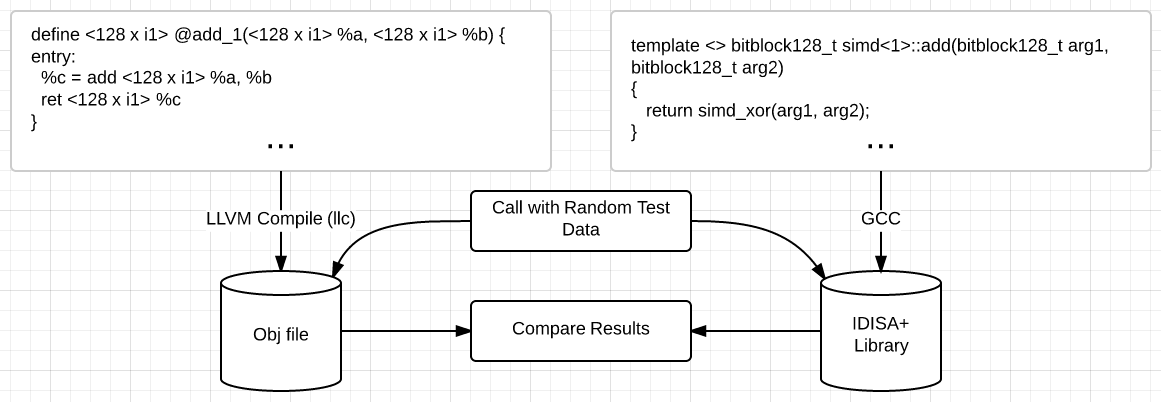
\includegraphics[width=140mm]{draw/test.png}
\caption[Test system overview.]{Test system overview. The pure IR library is first compiled into the native object file and then linked with the driver. The driver call functions from the both side to check correctness.}
\label{figure:test}
\end{figure}

\begin{program}
\begin{verbatim}

define <32 x i4> @{{name.c}}(<32 x i4> %a,
                             <32 x i4> %b)
{
entry:
  %c = {{ name.op }} <32 x i4> %a, %b
  
  %d = sext <32 x i1> %c to <32 x i4>
  ret <32 x i4> %d
  
  ret <32 x i4> %c
  
}

\end{verbatim}
\rule{\textwidth}{1pt}

\begin{multicols}{2}
\begin{verbatim}
define <32 x i4> @add_4(<32 x i4> %a,
                        <32 x i4> %b)
{
entry:
  %c = add <32 x i4> %a, %b
  ret <32 x i4> %c
}
\end{verbatim}
\columnbreak
\begin{verbatim}
define <32 x i4> @eq_4(<32 x i4> %a,
                       <32 x i4> %b)
{
entry:
  %c = icmp eq <32 x i4> %a, %b
  %d = sext <32 x i1> %c to <32 x i4>
  ret <32 x i4> %d
}
\end{verbatim}
\end{multicols}
\caption[Templates for the IR Libray]{Templates for the IR Library. On the top is the template, and two different output are listed below. We use embedded for loop and if statements.}
\label{program:jinja}
\end{program}
